\documentclass[]{article}

\usepackage[utf8]{inputenc}
\usepackage[T1]{fontenc}
\usepackage[english, french]{babel}

\usepackage{amsmath}
\usepackage{amssymb}
% \usepackage{mathrsfs}

\usepackage{hyperref}
\usepackage{scrextend}
\usepackage{xspace}

\usepackage{graphicx}

\usepackage{color}
\usepackage{listings}
\definecolor{listinggray}{gray}{0.9}
\definecolor{lbcolor}{rgb}{0.95,0.95,0.95}
\lstset{
	backgroundcolor=\color{lbcolor},
	tabsize=4,
	rulecolor=,
	language=Java,
	basicstyle=\scriptsize\ttfamily,
	upquote=false,
	aboveskip={.5\baselineskip},
	columns=fixed,
	showstringspaces=false,
	extendedchars=true,
	showspaces=false,
	breaklines=true,
	prebreak = \raisebox{0ex}[0ex][0ex]{\ensuremath{\hookleftarrow}},
	frame=single,
	showtabs=false,
	identifierstyle=\ttfamily,
	keywordstyle=\bfseries\color[rgb]{0,0,1},
	commentstyle=\color[rgb]{0.133,0.545,0.133},
	stringstyle=\color[rgb]{0.627,0.126,0.941},
}

\newcommand{\variable}[1]{\noindent \texttt{#1}}
\newcommand{\degr}[0]{$^\circ$}

%////////////////////////////////////////////////////////////////////////////////
%///////////////////////////PAGE DE GARDE////////////////////////////////
%//////////////////////////////////////////////////////////////////////////////
\title{Algo-Prog\\Sujet \no2 : Puzzle}
\author{Jeannin Émile, Mottet Théo}

\begin{document}

\maketitle
\newpage
\section{Mode d'emploi}

Le but du jeu est de reconstituer l'image dans la grille se trouvant à gauche de l'écran. Pour cela, le joueur peut cliquer sur une pièce, ce qui aura pour conséquence de voir la pièce suivre le curseur. Il faudra recliquer pour déposer la pièce. Si le curseur se trouve au dessus d'une des cases de la grille, l'image tenue sera déposée correctement dans la case (cela compte comme un coup).

Pour que le puzzle soit terminé, il faut que chaque pièce soit dans la bonne case et qu'elle ne soit pas tournée (la rotation de la pièce doit être de 0 degrés).

L'utilisateur peut tourner une piece de 90 degrés dans le sens des éguilles d'une montre en effectuant un clic droit sur une pièce. Cela a compte comme un coup.

A la fin du jeu, le temps est affiché ainsi que le nombre de coups que l'utilisateur a joué afin de résoudre le puzzle. On peut alors cliquer quelque part pour essayer un nouveau puzzle, ou bien simplement quitter l'application.

Enfin, plusieurs boutons sont à la disposition du joueur : pour changer de puzzle (aléatoirement), pour changer le nombre de pièces (a aussi pour effet de changer de puzzle) et pour activer/désactiver la rotation des pièces.

\section{Résolution des problèmes}

Problèmes (à mettre dans l'ordre):
\begin{itemize}
	\item
		Affichage (Tracage des pièces à l'écran, transparence, tjrs même fonction affichage, pzl passé en param);
	\item
		Placement des pièces dans la grille (Quand on clique au dessus d'une case en tenant une pièce, comment cell-ci est-elle positionnée dans la grille --> Est-elle au bon endroit ou non.);
	\item
		Condition de fin (Toutes les pièces placées correctement dans la grille, bonne rotation --> comment le sait-on?);
	\item
		Déplacement des pièces (Comment la pièce suit le curseur et est devant les autres, au premier clic, on tient l'image, au second on la lache);
	\item
		Rotation des pièces (Comment se passe la rotation : formule ; au clic droit, on lache l'image si on la tenait et on la fait tourner de 90$^\circ$);
	 \item
		Forme des pièces (Comment on fait les pics sur chaque côtés des images --> les pics sont complémentaires entre les images ; schéma pour comprendre);
	\item
		Clic (Systeme de gestion des clics pour simplifier leur utilisation --> Comment et pourquoi);
	\item
		Découpage de l'image (Comment on découpe l'image et pourquoi lors de l'initialisation);
	\item
		Boutons (Mise en place d'un systeme de création et d'affichage de boutons : comment il marche et pourquoi l'avoir fait);
	\item
		Nouvelle partie (Mise en place d'un système permettant de rejouer --> Comment ça marche);
	\item
		Bordures des pièces (On dessine un trait épais noir sur le bord extérieur du puzzle --> comment ça marche);
	\item
		Nombre de coups et temps (Les coups sont comptés et le temps aussi).
\end{itemize}

%////////////////////////////////////////////////////////////////////////////////
%///////////////////////////PREMIER CHAPITRE EMILE////////////////////
%//////////////////////////////////////////////////////////////////////////////

\subsection{Modification des pièces}

Dans cette partie, nous allons expliquer notre démarche pour tout ce qui a porté sur la modification des pièces, en particulier sur la modification de leur image.

Afin de pouvoir gérer la transparence d'une image, nous avons créé un type agrégé \variable{Pixel} qui permet à l'image d'avoir une composante alpha. Par la même occasion, nous avons créé la fonction \variable{drawImage} qui permet de tracer cette image à l'aide de la fonction \variable{EcranGraphique.drawPixel}. Les images seront donc des matrices de \variable{Pixel}.

\subsubsection{Bordures des pièces}

Pour que l'utilisateur du programme puisse facilement reconnaître les pièces qui sont en bordure du puzzle, nous avons décidé de tracer un contour noir de quelques pixels autour de l'image. Nous procédons donc avant le découpage de l'image. Dans la fonctionn \variable{saisirImage}, nous procédons ainsi :

\begin{lstlisting}
for(int j = 0; j < 5; j++)
{
    for(int i = 0; i < imgLarg; i++)
    {
        img[i][j] = 0;
        img[i][imgHaut - j - 1] = 0;
    }
}
\end{lstlisting}

Ce code permet de tracer deux lignes : une en haut de l'image, une au bas de l'image, chacune d'une largeur de 5 pixels. Nous utilisons le même principe pour tracer les deux lignes restantes, à gauche et à droite de l'image.

\subsubsection{Découpage de l'image}

Une fois l'image chargée, elle doit être découpée afin de constituer les pièces du puzzle. Pour cela, nous commençons par initialiser chaque pièces, ainsi que l'image de chaque pièce. La taille de l'image d'une pièce sera de 1.5 fois la largeur visible (de même en hauteur) car elle va posséder des bordures transparentes qui permettront d'ajouter des dents sur les pièces.

Le découpage de l'image est plutôt simple car il s'agit en fait d'une copie de chaque pixel de l'image chargée dans la case correspondante (voir code). Mais on pense aux bordures pour centrer l'image visible soit centrée dans le tableau de pixels. Les pixels non attribués lors de cette copie devront être transparent.

\subsubsection{Rotation des pièces}

Dans le cas où \variable{rotation} est vrai, donc dans le cas où la rotation est activée, les pièces doivent pouvoir tourner de 90\degr lorsqu'on effectue un clic droit dessus.

Ainsi, dans la fonction \variable{jouerCoup}, si il y a un clic droit et que ce clic droit est sur une pièce, on fait pivoter cette dernière et on fini le tour. Ceci a pour effet de lâcher la pièce tenue (si il y en avait une) et d'incrémenter le nombre de coups utilisés par le joueur.

Nous avons créé une fonction \variable{pivoterImage} qui permet de tourner une pièce de 90\degr. Cette fonction indiquera que la pièce a été tournée en ajoutant 90 à la variable \variable{rotation} de la pièce en question et fera pivoter l'image. Dans le but de tourner l'image, nous avons besoin de changer la position de chacun de ses pixels. Pour cela, nous copions l'image dans une image temporaire (\variable{Pixel imgTrans[][]}). Nous pourrons ainsi réattribuer chaque pixel correctement.

L'image étant une matrice, pour la faire pivoter, nous procédons ainsi : le pixel se trouvant à la position (i, j) -- i le numéro de colonne et j le numéro de ligne -- devra se trouver à la position (n - j, i) avec n la largeur/hauteur de l'image.

Après avoir effectué cette opération avec chaque pixel, l'image aura bien été pivotée de 90\degr.

\subsubsection{Formes des pièces}

\begin{figure}[hpt]
	\center
	\caption{\label{Forme des pièces} Forme des pièces}
	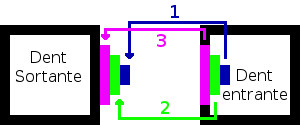
\includegraphics{dents}
\end{figure}

Nous avons créé une fonction \variable{bords} qui permet de créer les dents sur chaque côté des pièces. Cette fonction va simplement parcourir le tableaux des pièces du puzzle et appeler les fonctions \variable{bordsVertic} et \variable{bordsHoriz}. Ces dernières vont créer une dent entrante dans une pièce et une dent sortante dans l'autre. Les deux pièces passées en paramètre de ces fonctions doivent donc être côte à côte (la première dessus la deuxième pour \variable{bordsVertic} et la première à gauche de la deuxième pour \variable{bordsHoriz}).

Pour pouvoir ajouter des dents sortantes aux pièces, nous avons agrandi la taille de leur image, en placant tout autour de l'image visible un contour transparent (de largeur 1/4 de la taille de l'image visible). Ainsi, on va pouvoir changer la couleur de certains pixels transparents pour afficher une dent sortante. Pour afficher une dent entrante, il suffira de rendre certains pixels transparents.

Voici comment nous procédons pour créer une dent (ici, une dent sortante à gauche et donc entrante à droite mais le principe est identique pour les autres cas de figure) : nous copions le pixel qui est au centre de l'image de droite (verticalement) et qui est horizontalement à 1/2 de la taille de l'image visible (la bordure faisant 1/4 et on veut le pixel à la pointe du triangle), et nous le plaçons sur l'image de gauche au milieu verticalement et au dernier pixel de l'image horizontalement. Le pixel à droite sera défini transparent pour créer la dent entrante. Nous continuons ainsi de suite, mais avec 3 pixels, puis 5... jusqu'à obtenir un triangle (voir code).

%////////////////////////////////////////////////////////////////////////////////
%///////////////////////////DEUXIEME CHAPITRE THEO //////////////////
%//////////////////////////////////////////////////////////////////////////////

\subsection{Ergonomie}
\subsubsection{Placement des pièces}

Pour placer les pièces nous avons procéder en différentes étapes. Dans un premier temps nous avons utilisé 4 booléens : 
\begin{lstlisting}
// Si il y a eu un clic (donc si on a une piece en main)
boolean pieceTenue = false;
// Si le tour est fini
boolean finDuCoup = false;
// Si on veut changer de puzzle
boolean relancer = false;
// Passe a true si il y a un clic (n'importe lequel)
 boolean unClic;
\end{lstlisting}
Ainsi, nous pouvons vérifier quand le clic de la souris est utilisé. 
Pour ce faire, on met à jour l'état de la souris à chaque tour de boucle. On regarde si il s'agit d'un clic gauche et on vérifie que la pièce est bien en main grâce au booléen \variable{pieceTenue}.

\subsubsection{Boutons}
\subsubsection{Gestion des clics}

%///////////////////////////////////////////////////////////////////////////////
%///////////////////////////TROISIEME CHAPITRE THEO/////////////////
%//////////////////////////////////////////////////////////////////////////////

\subsection{Gameplay}
\subsubsection{Nombres de coups et temps}
\subsubsection{Nouvelle partie}
\subsubsection{Condition de fin}

%/////////////////////////////////////////////////////////////////////////////////
%///////////////////////////QUATRIEME CHAPITRE EMILE/////////////////
%//////////////////////////////////////////////////////////////////////////////

\subsection{Affichage et déplacements}

Cette partie décrira comment nous avons résolu la question de l'affichage et du déplacement des pièces.

\subsubsection{Déplacement des pièces}

Nous avons décidé que la pièce suivrait le curseur lorsqu'elle est sélectionnée. Pour cela, nous vérifions (dans la fonction \variable{jouerCoup} que l'utilisateur effectue un clic gauche sur une pièce et qu'il n'y avait pas de pièces tenue à ce moment. Si l'utilisateur avait dans la main une pièce, elle sera posée par cette action. Donc après un clic sur une pièce, la pièce en question va suivre le curseur. En effet, cette pièce est identifiée par \variable{pzl.caseChoisie} avec \variable{pzl} notre variable \variable{PuzzleJeu} contenant le puzzle entier et \variable{caseChoisie} qui est une position : celle de la case tenue par l'utilisateur.

À chaque tour de boucle, nous mettons à jour la position de la pièce correspondant à \variable{caseChoisie} (uniquement si caseChoisie est valide : si aucune case n'est tenue, \variable{caseChoisie.x = -1} et \variable{caseChoisie.y = -1}. Le curseur doit se trouver au centre de l'image, la position sera donc affectée en conséquence.

Enfin, dans l'affichage, cette case devra être affichée après les autrespour ne pas qu'elle soit visuellement en dessous d'une autre lorsqu'on la déplace (et qu'on puisse ainsi déduire sa véritable position dans la grille).

\subsubsection{Affichage}

Nous avons décidé de créer une fonction affichage qui gérera tout l'affichage du puzzle. Pour cela, nous lui envoyons notre variable principale \variable{PuzzleJeu pzl}.

La première étape est de nétoyer l'écran, c'est à dire d'exécuter : 
\begin{lstlisting}
EcranGraphique.clear();
\end{lstlisting}

Ensuite, nous dessinons la grille : des lignes horizontales et des lignes verticales du même nombre de pizels que l'image (en largeur ou hauteur), et nous traçons également les instructions du jeu : quelques règles.

Vient ensuite l'affichage des pièces : l'image contenue dans celles-ci est tracée (image qui a pu être tournée préalablement), mais on prend soin de ne pas tracer l'image tenue (si il y en a une). Nous ne dessinons qu'ensuite l'image tenue,afin qu'elle soit affichée au dessus des autres.

Nous traçons ensuite le texte de réussite si le puzzle est fini, puis nous affichons le menu (avec ses différents boutons) et des textes d'aide pour chaque bouton).

On termine la fonction en affichant le tout à l'écran. 

%/////////////////////////////////////////////////////////////////////////////////
%///////////////////////////INDEX/////////////////////////////////////////////
%//////////////////////////////////////////////////////////////////////////////

\newpage
\tableofcontents

\end{document}